\documentclass[12pt]{article}

% a template that a friend gave, it's worked well enough for me
% i have added some packages and stuff that have proved useful

\usepackage{fancyhdr}
\usepackage{tipa}
\usepackage{fontspec}
\usepackage{amsfonts}
\usepackage{enumitem}
\usepackage[margin=1in]{geometry}
\usepackage{graphicx}
\usepackage{float}
\usepackage{amsmath}
\usepackage{braket}
\usepackage{amssymb}
\usepackage{booktabs}
\usepackage{hyperref}
\usepackage{mathtools}
\usepackage{xcolor}
\usepackage{float}
\usepackage{algpseudocodex}
\usepackage{titlesec}
\usepackage{bbm}

\pagestyle{fancy}
\fancyhf{} % sets both header and footer to nothing
\lhead{Kevin Sheng}
\setmainfont{Comic Neue}
\renewcommand{\headrulewidth}{1pt}
\setlength{\headheight}{0.75in}
\setlength{\oddsidemargin}{0in}
\setlength{\evensidemargin}{0in}
\setlength{\voffset}{-.5in}
\setlength{\headsep}{10pt}
\setlength{\textwidth}{6.5in}
\setlength{\headwidth}{6.5in}
\setlength{\textheight}{8in}
\renewcommand{\headrulewidth}{0.5pt}
\renewcommand{\footrulewidth}{0.3pt}
\setlength{\textwidth}{6.5in}
\usepackage{setspace}
\usepackage{multicol}
\usepackage{float}
\setlength{\columnsep}{1cm}
\setlength\parindent{24pt}
\usepackage [english]{babel}
\usepackage [autostyle, english = american]{csquotes}
\MakeOuterQuote{"}

\setlength{\parskip}{6pt}
\setlength{\parindent}{0pt}

\titlespacing\section{0pt}{12pt plus 4pt minus 2pt}{0pt plus 2pt minus 2pt}
\titlespacing\subsection{0pt}{12pt plus 4pt minus 2pt}{0pt plus 2pt minus 2pt}
\titlespacing\subsubsection{0pt}{12pt plus 4pt minus 2pt}{0pt plus 2pt minus 2pt}

\hypersetup{colorlinks=true, urlcolor=blue}

\newcommand{\correction}[1]{\textcolor{red}{#1}}


\rhead{Math 180}

\makeatletter
\def\@seccntformat#1{%
  \expandafter\ifx\csname c@#1\endcsname\c@section\else
  \csname the#1\endcsname\quad
  \fi}
\makeatother

\newcommand{\Mod}[1]{\ (\mathrm{mod}\ #1)}

\begin{document}

\section{Chapter 5.1}

\begin{enumerate}
      \item[6] The proof is by induction.
      For $n=2$, there's only one possible tree and it has two leaves,
      so $p_1=2$ and the proposition is satisfied.
      Assuming truth for $n$, we now try to prove the validity of the statement for $n+1$.

      By what was proved in class, we can construct any tree with $n+1$ nodes
      just by adding a leaf to an existing tree with just $n$ nodes.
      Suppose the node we add the leaf onto has degree $d$.

      Notice that adding a leaf to this node increases its degree by $1$,
      so now $p_d$ decreases by $1$ and $p_{d+1}$ increases by $1$.
      By how we defined the summation, this makes the overall
      sum on the RHS decrease by $1$, since
      \[-(d-2)p_d-(d-1)p_{d+1}=-(d-2)(p_d-1)-(d-1)(p_{d+1}+1)+1\]

      However, we still have to add the leaf, which
      does nothing but increase $p_1$ and the total sum by $1$.
      The decrement and the increment balance each other out,
      so no matter what the sum of the expression stays at $2$. $\square$
\end{enumerate}

\pagebreak

\section{Chapter 5.2}

\begin{enumerate}
      \item[2] Although the two trees below have the same degree sequence,
      they aren't isomorphic since the "junctions" are at a different distance from each other.
      \begin{center}
            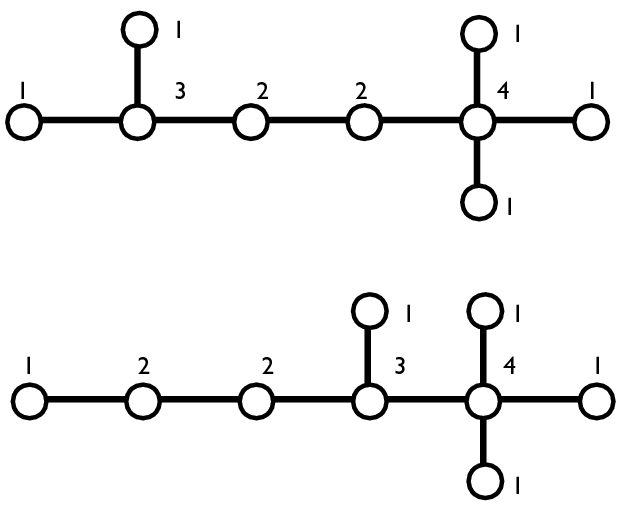
\includegraphics[width=10cm]{img/hw3/same_score}
      \end{center}

      \item[6] Represent each tree with the $01$-encoding taught in class.
      Each node contributes two characters to the string, so let's just
      stupidly consider all binary strings of length $2n$.
      Each character has two possible values, so there's $2^{2n}=4^n$ encodings.
      Though not all of them are valid, we're just trying to prove
      an upper bound here. $\square$
\end{enumerate}


\end{document}
